
%% bare_jrnl.tex
%% V1.4b
%% 2015/08/26
%% by Michael Shell
%% see http://www.michaelshell.org/
%% for current contact information.
%%
%% This is a skeleton file demonstrating the use of IEEEtran.cls
%% (requires IEEEtran.cls version 1.8b or later) with an IEEE
%% journal paper.
%%
%% Support sites:
%% http://www.michaelshell.org/tex/ieeetran/
%% http://www.ctan.org/pkg/ieeetran
%% and
%% http://www.ieee.org/

%%*************************************************************************
%% Legal Notice:
%% This code is offered as-is without any warranty either expressed or
%% implied; without even the implied warranty of MERCHANTABILITY or
%% FITNESS FOR A PARTICULAR PURPOSE! 
%% User assumes all risk.
%% In no event shall the IEEE or any contributor to this code be liable for
%% any damages or losses, including, but not limited to, incidental,
%% consequential, or any other damages, resulting from the use or misuse
%% of any information contained here.
%%
%% All comments are the opinions of their respective authors and are not
%% necessarily endorsed by the IEEE.
%%
%% This work is distributed under the LaTeX Project Public License (LPPL)
%% ( http://www.latex-project.org/ ) version 1.3, and may be freely used,
%% distributed and modified. A copy of the LPPL, version 1.3, is included
%% in the base LaTeX documentation of all distributions of LaTeX released
%% 2003/12/01 or later.
%% Retain all contribution notices and credits.
%% ** Modified files should be clearly indicated as such, including  **
%% ** renaming them and changing author support contact information. **
%%*************************************************************************


% *** Authors should verify (and, if needed, correct) their LaTeX system  ***
% *** with the testflow diagnostic prior to trusting their LaTeX platform ***
% *** with production work. The IEEE's font choices and paper sizes can   ***
% *** trigger bugs that do not appear when using other class files.       ***                          ***
% The testflow support page is at:
% http://www.michaelshell.org/tex/testflow/



\documentclass[journal,a4paper,pdftex]{IEEEtran}
\usepackage{tcolorbox}
\usepackage{lipsum}
\usepackage{cuted}
\usepackage{fancyvrb}
%
% If IEEEtran.cls has not been installed into the LaTeX system files,
% manually specify the path to it like:
% \documentclass[journal]{../sty/IEEEtran}





% Some very useful LaTeX packages include:
% (uncomment the ones you want to load)


% *** MISC UTILITY PACKAGES ***
%
%\usepackage{ifpdf}
% Heiko Oberdiek's ifpdf.sty is very useful if you need conditional
% compilation based on whether the output is pdf or dvi.
% usage:
% \ifpdf
%   % pdf code
% \else
%   % dvi code
% \fi
% The latest version of ifpdf.sty can be obtained from:
% http://www.ctan.org/pkg/ifpdf
% Also, note that IEEEtran.cls V1.7 and later provides a builtin
% \ifCLASSINFOpdf conditional that works the same way.
% When switching from latex to pdflatex and vice-versa, the compiler may
% have to be run twice to clear warning/error messages.






% *** CITATION PACKAGES ***
%
%\usepackage{cite}
% cite.sty was written by Donald Arseneau
% V1.6 and later of IEEEtran pre-defines the format of the cite.sty package
% \cite{} output to follow that of the IEEE. Loading the cite package will
% result in citation numbers being automatically sorted and properly
% "compressed/ranged". e.g., [1], [9], [2], [7], [5], [6] without using
% cite.sty will become [1], [2], [5]--[7], [9] using cite.sty. cite.sty's
% \cite will automatically add leading space, if needed. Use cite.sty's
% noadjust option (cite.sty V3.8 and later) if you want to turn this off
% such as if a citation ever needs to be enclosed in parenthesis.
% cite.sty is already installed on most LaTeX systems. Be sure and use
% version 5.0 (2009-03-20) and later if using hyperref.sty.
% The latest version can be obtained at:
% http://www.ctan.org/pkg/cite
% The documentation is contained in the cite.sty file itself.



% *** GRAPHICS RELATED PACKAGES ***
%
\ifCLASSINFOpdf
  \usepackage[pdftex]{graphicx}
  % declare the path(s) where your graphic files are
   \graphicspath{{./pdf/}{./jpeg/}}
  % and their extensions so you won't have to specify these with
  % every instance of \includegraphics
  \DeclareGraphicsExtensions{.pdf,.jpg,.png}
\else
  % or other class option (dvipsone, dvipdf, if not using dvips). graphicx
  % will default to the driver specified in the system graphics.cfg if no
  % driver is specified.
  % \usepackage[dvips]{graphicx}
  % declare the path(s) where your graphic files are
  % \graphicspath{{../eps/}}
  % and their extensions so you won't have to specify these with
  % every instance of \includegraphics
  % \DeclareGraphicsExtensions{.eps}
\fi
% graphicx was written by David Carlisle and Sebastian Rahtz. It is
% required if you want graphics, photos, etc. graphicx.sty is already
% installed on most LaTeX systems. The latest version and documentation
% can be obtained at: 
% http://www.ctan.org/pkg/graphicx
% Another good source of documentation is "Using Imported Graphics in
% LaTeX2e" by Keith Reckdahl which can be found at:
% http://www.ctan.org/pkg/epslatex
%
% latex, and pdflatex in dvi mode, support graphics in encapsulated
% postscript (.eps) format. pdflatex in pdf mode supports graphics
% in .pdf, .jpeg, .png and .mps (metapost) formats. Users should ensure
% that all non-photo figures use a vector format (.eps, .pdf, .mps) and
% not a bitmapped formats (.jpeg, .png). The IEEE frowns on bitmapped formats
% which can result in "jaggedy"/blurry rendering of lines and letters as
% well as large increases in file sizes.
%
% You can find documentation about the pdfTeX application at:
% http://www.tug.org/applications/pdftex





% *** MATH PACKAGES ***
%
%\usepackage{amsmath}
% A popular package from the American Mathematical Society that provides
% many useful and powerful commands for dealing with mathematics.
%
% Note that the amsmath package sets \interdisplaylinepenalty to 10000
% thus preventing page breaks from occurring within multiline equations. Use:
%\interdisplaylinepenalty=2500
% after loading amsmath to restore such page breaks as IEEEtran.cls normally
% does. amsmath.sty is already installed on most LaTeX systems. The latest
% version and documentation can be obtained at:
% http://www.ctan.org/pkg/amsmath





% *** SPECIALIZED LIST PACKAGES ***
%
%\usepackage{algorithmic}
% algorithmic.sty was written by Peter Williams and Rogerio Brito.
% This package provides an algorithmic environment fo describing algorithms.
% You can use the algorithmic environment in-text or within a figure
% environment to provide for a floating algorithm. Do NOT use the algorithm
% floating environment provided by algorithm.sty (by the same authors) or
% algorithm2e.sty (by Christophe Fiorio) as the IEEE does not use dedicated
% algorithm float types and packages that provide these will not provide
% correct IEEE style captions. The latest version and documentation of
% algorithmic.sty can be obtained at:
% http://www.ctan.org/pkg/algorithms
% Also of interest may be the (relatively newer and more customizable)
% algorithmicx.sty package by Szasz Janos:
% http://www.ctan.org/pkg/algorithmicx




% *** ALIGNMENT PACKAGES ***
%
%\usepackage{array}
% Frank Mittelbach's and David Carlisle's array.sty patches and improves
% the standard LaTeX2e array and tabular environments to provide better
% appearance and additional user controls. As the default LaTeX2e table
% generation code is lacking to the point of almost being broken with
% respect to the quality of the end results, all users are strongly
% advised to use an enhanced (at the very least that provided by array.sty)
% set of table tools. array.sty is already installed on most systems. The
% latest version and documentation can be obtained at:
% http://www.ctan.org/pkg/array


% IEEEtran contains the IEEEeqnarray family of commands that can be used to
% generate multiline equations as well as matrices, tables, etc., of high
% quality.




% *** SUBFIGURE PACKAGES ***
%\ifCLASSOPTIONcompsoc
%  \usepackage[caption=false,font=normalsize,labelfont=sf,textfont=sf]{subfig}
%\else
%  \usepackage[caption=false,font=footnotesize]{subfig}
%\fi
% subfig.sty, written by Steven Douglas Cochran, is the modern replacement
% for subfigure.sty, the latter of which is no longer maintained and is
% incompatible with some LaTeX packages including fixltx2e. However,
% subfig.sty requires and automatically loads Axel Sommerfeldt's caption.sty
% which will override IEEEtran.cls' handling of captions and this will result
% in non-IEEE style figure/table captions. To prevent this problem, be sure
% and invoke subfig.sty's "caption=false" package option (available since
% subfig.sty version 1.3, 2005/06/28) as this is will preserve IEEEtran.cls
% handling of captions.
% Note that the Computer Society format requires a larger sans serif font
% than the serif footnote size font used in traditional IEEE formatting
% and thus the need to invoke different subfig.sty package options depending
% on whether compsoc mode has been enabled.
%
% The latest version and documentation of subfig.sty can be obtained at:
% http://www.ctan.org/pkg/subfig




% *** FLOAT PACKAGES ***
%
%\usepackage{fixltx2e}
% fixltx2e, the successor to the earlier fix2col.sty, was written by
% Frank Mittelbach and David Carlisle. This package corrects a few problems
% in the LaTeX2e kernel, the most notable of which is that in current
% LaTeX2e releases, the ordering of single and double column floats is not
% guaranteed to be preserved. Thus, an unpatched LaTeX2e can allow a
% single column figure to be placed prior to an earlier double column
% figure.
% Be aware that LaTeX2e kernels dated 2015 and later have fixltx2e.sty's
% corrections already built into the system in which case a warning will
% be issued if an attempt is made to load fixltx2e.sty as it is no longer
% needed.
% The latest version and documentation can be found at:
% http://www.ctan.org/pkg/fixltx2e


%\usepackage{stfloats}
% stfloats.sty was written by Sigitas Tolusis. This package gives LaTeX2e
% the ability to do double column floats at the bottom of the page as well
% as the top. (e.g., "\begin{figure*}[!b]" is not normally possible in
% LaTeX2e). It also provides a command:
%\fnbelowfloat
% to enable the placement of footnotes below bottom floats (the standard
% LaTeX2e kernel puts them above bottom floats). This is an invasive package
% which rewrites many portions of the LaTeX2e float routines. It may not work
% with other packages that modify the LaTeX2e float routines. The latest
% version and documentation can be obtained at:
% http://www.ctan.org/pkg/stfloats
% Do not use the stfloats baselinefloat ability as the IEEE does not allow
% \baselineskip to stretch. Authors submitting work to the IEEE should note
% that the IEEE rarely uses double column equations and that authors should try
% to avoid such use. Do not be tempted to use the cuted.sty or midfloat.sty
% packages (also by Sigitas Tolusis) as the IEEE does not format its papers in
% such ways.
% Do not attempt to use stfloats with fixltx2e as they are incompatible.
% Instead, use Morten Hogholm'a dblfloatfix which combines the features
% of both fixltx2e and stfloats:
%
% \usepackage{dblfloatfix}
% The latest version can be found at:
% http://www.ctan.org/pkg/dblfloatfix




%\ifCLASSOPTIONcaptionsoff
%  \usepackage[nomarkers]{endfloat}
% \let\MYoriglatexcaption\caption
% \renewcommand{\caption}[2][\relax]{\MYoriglatexcaption[#2]{#2}}
%\fi
% endfloat.sty was written by James Darrell McCauley, Jeff Goldberg and 
% Axel Sommerfeldt. This package may be useful when used in conjunction with 
% IEEEtran.cls'  captionsoff option. Some IEEE journals/societies require that
% submissions have lists of figures/tables at the end of the paper and that
% figures/tables without any captions are placed on a page by themselves at
% the end of the document. If needed, the draftcls IEEEtran class option or
% \CLASSINPUTbaselinestretch interface can be used to increase the line
% spacing as well. Be sure and use the nomarkers option of endfloat to
% prevent endfloat from "marking" where the figures would have been placed
% in the text. The two hack lines of code above are a slight modification of
% that suggested by in the endfloat docs (section 8.4.1) to ensure that
% the full captions always appear in the list of figures/tables - even if
% the user used the short optional argument of \caption[]{}.
% IEEE papers do not typically make use of \caption[]'s optional argument,
% so this should not be an issue. A similar trick can be used to disable
% captions of packages such as subfig.sty that lack options to turn off
% the subcaptions:
% For subfig.sty:
% \let\MYorigsubfloat\subfloat
% \renewcommand{\subfloat}[2][\relax]{\MYorigsubfloat[]{#2}}
% However, the above trick will not work if both optional arguments of
% the \subfloat command are used. Furthermore, there needs to be a
?
% description of each subfigure *somewhere* and endfloat does not add
% subfigure captions to its list of figures. Thus, the best approach is to
% avoid the use of subfigure captions (many IEEE journals avoid them anyway)
% and instead reference/explain all the subfigures within the main caption.
% The latest version of endfloat.sty and its documentation can obtained at:
% http://www.ctan.org/pkg/endfloat
%
% The IEEEtran \ifCLASSOPTIONcaptionsoff conditional can also be used
% later in the document, say, to conditionally put the References on a 
% page by themselves.




% *** PDF, URL AND HYPERLINK PACKAGES ***
%
%\usepackage{url}
% url.sty was written by Donald Arseneau. It provides better support for
% handling and breaking URLs. url.sty is already installed on most LaTeX
% systems. The latest version and documentation can be obtained at:
% http://www.ctan.org/pkg/url
% Basically, \url{my_url_here}.




% *** Do not adjust lengths that control margins, column widths, etc. ***
% *** Do not use packages that alter fonts (such as pslatex).         ***
% There should be no need to do such things with IEEEtran.cls V1.6 and later.
% (Unless specifically asked to do so by the journal or conference you plan
% to submit to, of course. )


% correct bad hyphenation here
\hyphenation{op-tical net-works semi-conduc-tor}
\includeonly{introduction}

\begin{document}
%
% paper title
% Titles are generally capitalized except for words such as a, an, and, as,
% at, but, by, for, in, nor, of, on, or, the, to and up, which are usually
% not capitalized unless they are the first or last word of the title.
% Linebreaks \\ can be used within to get better formatting as desired.
% Do not put math or special symbols in the title.
\title{Bare Demo of IEEEtran.cls\\ for IEEE Journals}
%
%
% author names and IEEE memberships
% note positions of commas and nonbreaking spaces ( ~ ) LaTeX will not break
% a structure at a ~ so this keeps an author's name from being broken across
% two lines.
% use \thanks{} to gain access to the first footnote area
% a separate \thanks must be used for each paragraph as LaTeX2e's \thanks
% was not built to handle multiple paragraphs
%

\author{Ranganai Mapondera\\Pawsey Supercomputing Centre Curtin University Perth, Australia\\Email:ranganai.mapondera@student.curtin.edu.au}
\author{Ozlem Erkilic\\Pawsey Supercomputing Centre Curtin University\\Perth, Australia\\Email:ozlem.erkilic@student.curtin.edu.au}

%\author{Michael~Shell,~\IEEEmembership{Member,~IEEE,}
       % John~Doe,~\IEEEmembership{Fellow,~OSA,}
       % and~Jane~Doe,~\IEEEmembership{Life~Fellow,~IEEE}% <-this % stops a space
%\thanks{M. Shell was with the Department
%of Electrical and Computer Engineering, Georgia Institute of Technology, Atlanta,
%GA, 30332 USA e-mail: (see http://www.michaelshell.org/contact.html).}% <-this % stops a space
%\thanks{J. Doe and J. Doe are with Anonymous University.}% <-this % stops a space
%\thanks{Manuscript received April 19, 2005; revised August 26, 2015.}}

% note the % following the last \IEEEmembership and also \thanks - 
% these prevent an unwanted space from occurring between the last author name
% and the end of the author line. i.e., if you had this:
% 
% \author{....lastname \thanks{...} \thanks{...} }
%                     ^------------^------------^----Do not want these spaces!
%
% a space would be appended to the last name and could cause every name on that
% line to be shifted left slightly. This is one of those "LaTeX things". For
% instance, "\textbf{A} \textbf{B}" will typeset as "A B" not "AB". To get
% "AB" then you have to do: "\textbf{A}\textbf{B}"
% \thanks is no different in this regard, so shield the last } of each \thanks
% that ends a line with a % and do not let a space in before the next \thanks.
% Spaces after \IEEEmembership other than the last one are OK (and needed) as
% you are supposed to have spaces between the names. For what it is worth,
% this is a minor point as most people would not even notice if the said evil
% space somehow managed to creep in.



% The paper headers
\markboth{Proceedings of the Pawsey Supercomputing Centre Summer Internships,~Vol.~1, No.~1, February~2017}%
{Shell \MakeLowercase{\textit{et al.}}: Demo of IEEEtran.cls for Pawsey Internships}
% The only time the second header will appear is for the odd numbered pages
% after the title page when using the twoside option.
% 
% *** Note that you probably will NOT want to include the author's ***
% *** name in the headers of peer review papers.                   ***
% You can use \ifCLASSOPTIONpeerreview for conditional compilation here if
% you desire.




% If you want to put a publisher's ID mark on the page you can do it like
% this:
%\IEEEpubid{0000--0000/00\$00.00~\copyright~2015 IEEE}
% Remember, if you use this you must call \IEEEpubidadjcol in the second
% column for its text to clear the IEEEpubid mark.



% use for special paper notices
%\IEEEspecialpapernotice{(Invited Paper)}




% make the title area
\maketitle

% As a general rule, do not put math, special symbols or citations
% in the abstract or keywords.
\begin{abstract}
The best way to understand how to compute a task based on some resources, constraints and goals on advanced computing systems is to work through sample 
codes. A lot of expert users browse through the Internet to find these examples that they can slightly modify to achieve the results they expect. 
However, this can be very diffucult for some users who are new to this environment as there are always so many of these examples which are not 
always what they specifically need. This brings out the challenge of having to modify the example to suit their requirements on a particular computing 
resource, mainly the High Performance Computing systems (HPC) since the modified examples mostly do not work due to HPC systems having different set ups.
Therefore, it is hard to tell what the issue is for inexperienced users. Quite often, the users maynot be able to tell if the example is broken or if 
the example is correct, but maybe the code requires some adjustments. This is a very common issue encountered by the users of Pawsey Supercomputing 
Centre. For this reason, this paper provides solutions to how to run and submit examples on different resources such as supercomputers of Pawsey 
Supercomputing Centre through the use of a simple tool "getexample". The "getexample" is an effective tool that is developed for the supercomputers of 
Pawsey that are dependent on a command line interface and aims to help their users learn to how to run code mainly parallel programming examples, submit 
these examples to different operating systems of Pawsey such as Magnus, Zeus and Zythos. Although, the getexample is limited to these HPC resources, it 
has the potential to be expanded to other resources and interfaces. 
\end{abstract}

% Note that keywords are not normally used for peerreview papers.
\begin{IEEEkeywords}
IEEE, IEEEtran, journal, \LaTeX, paper, template.
\end{IEEEkeywords}






% For peer review papers, you can put extra information on the cover
% page as needed:
% \ifCLASSOPTIONpeerreview
% \begin{center} \bfseries EDICS Category: 3-BBND \end{center}
% \fi
%
% For peerreview papers, this IEEEtran command inserts a page break and
% creates the second title. It will be ignored for other modes.
\IEEEpeerreviewmaketitle


\section{Introduction}

\IEEEPARstart{E}{ven} though there are many sample codes on search engines for programming purposes, it is usually very rare that these codes work at 
the first try on different high performance computing systems without modifying them. This is mainly due to each advanced computing system being built 
up differently from each other to perform specific tasks for the needs of the users. At Pawsey Supercomputing Centre, there are various HPC resources 
where each of them are set up with slight variations from each other. Therefore, this becomes very challanging for the users, especially the beginners 
to change the example codes to display a working task on Pawsey's resources as there are many differences between each resources with many constraints. 
The most common differences between their systems are as follows:

\begin{itemize}
\item The operating systems
\item The clusters such as homogeneous or heterogeneouos
\item The program environments
\item The compiler options with varying commands
\item The compiler flags and wrappers for varying compiler options
\item The Module systems and paths 
\item The library versions
\item The personal scratch, group and home directories
\item The scheduling policies
\end{itemize}

For this reason, when the user runs a sample code found from the Internet for each supercomputers (Magnus, Zeus and Zythos), the code fails to compile 
as expected and hence, does not run as each individual system has specific operating system and commands set up for them. To rectify these problems, 
some HPC resources provide their users websites with working examples that aim to assist them how to carry out their tasks step by step. 
However, sometimes the commands in these examples can be outdated due to the updates in compilers and the operating systems. They also can be challenging 
to follow and perform on the real systems for the users who are not very experienced with these resources. Although, one may find a well-written bash 
script to run these systems, may not know how to make this script executable by changing the permissions using the chmod commands. Furthermore, a user 
may use a sample source code such as a basic MPI code which includes some MPI libraries to perform a particular job on these supercomputers but may 
fail when compiled due to these libraries being no longer valid or upgraded to a different version. Or one may complete their task, but may 
not know in which filesystem to store their results, for example in scratch or their group because some supercomputers have policies on how long to keep 
the data on certain filesystems such as scratch. If they are not moved from that specific file system within a certain amount of time, the results get 
deleted and thus, the user loses their work. This is a major difficulty for the users, especially researchers and scientist since it takes very long time 
to collect their data. It is also very crucial that these are stored correctly within these sources.

In order to minimise these problems, the getexample was developed to supply examples which do not require further editing or modification and works
when the executable is run. Thus, it aims to teach the users of Pawsey Supercomputing Centre how to run and submit tasks on the supercomputers without 
encountering issues. The rest of this paper explains how the getexample tool works.   

\begin{figure}[!ht]
\begin{center}
\includegraphics[height=4cm,width=4cm]{getexamplemagnus}
\caption{elastic data set 1}
\label{dataset1}
\end{center}
\end{figure} 

\begin{figure}[!hb]
\begin{center}
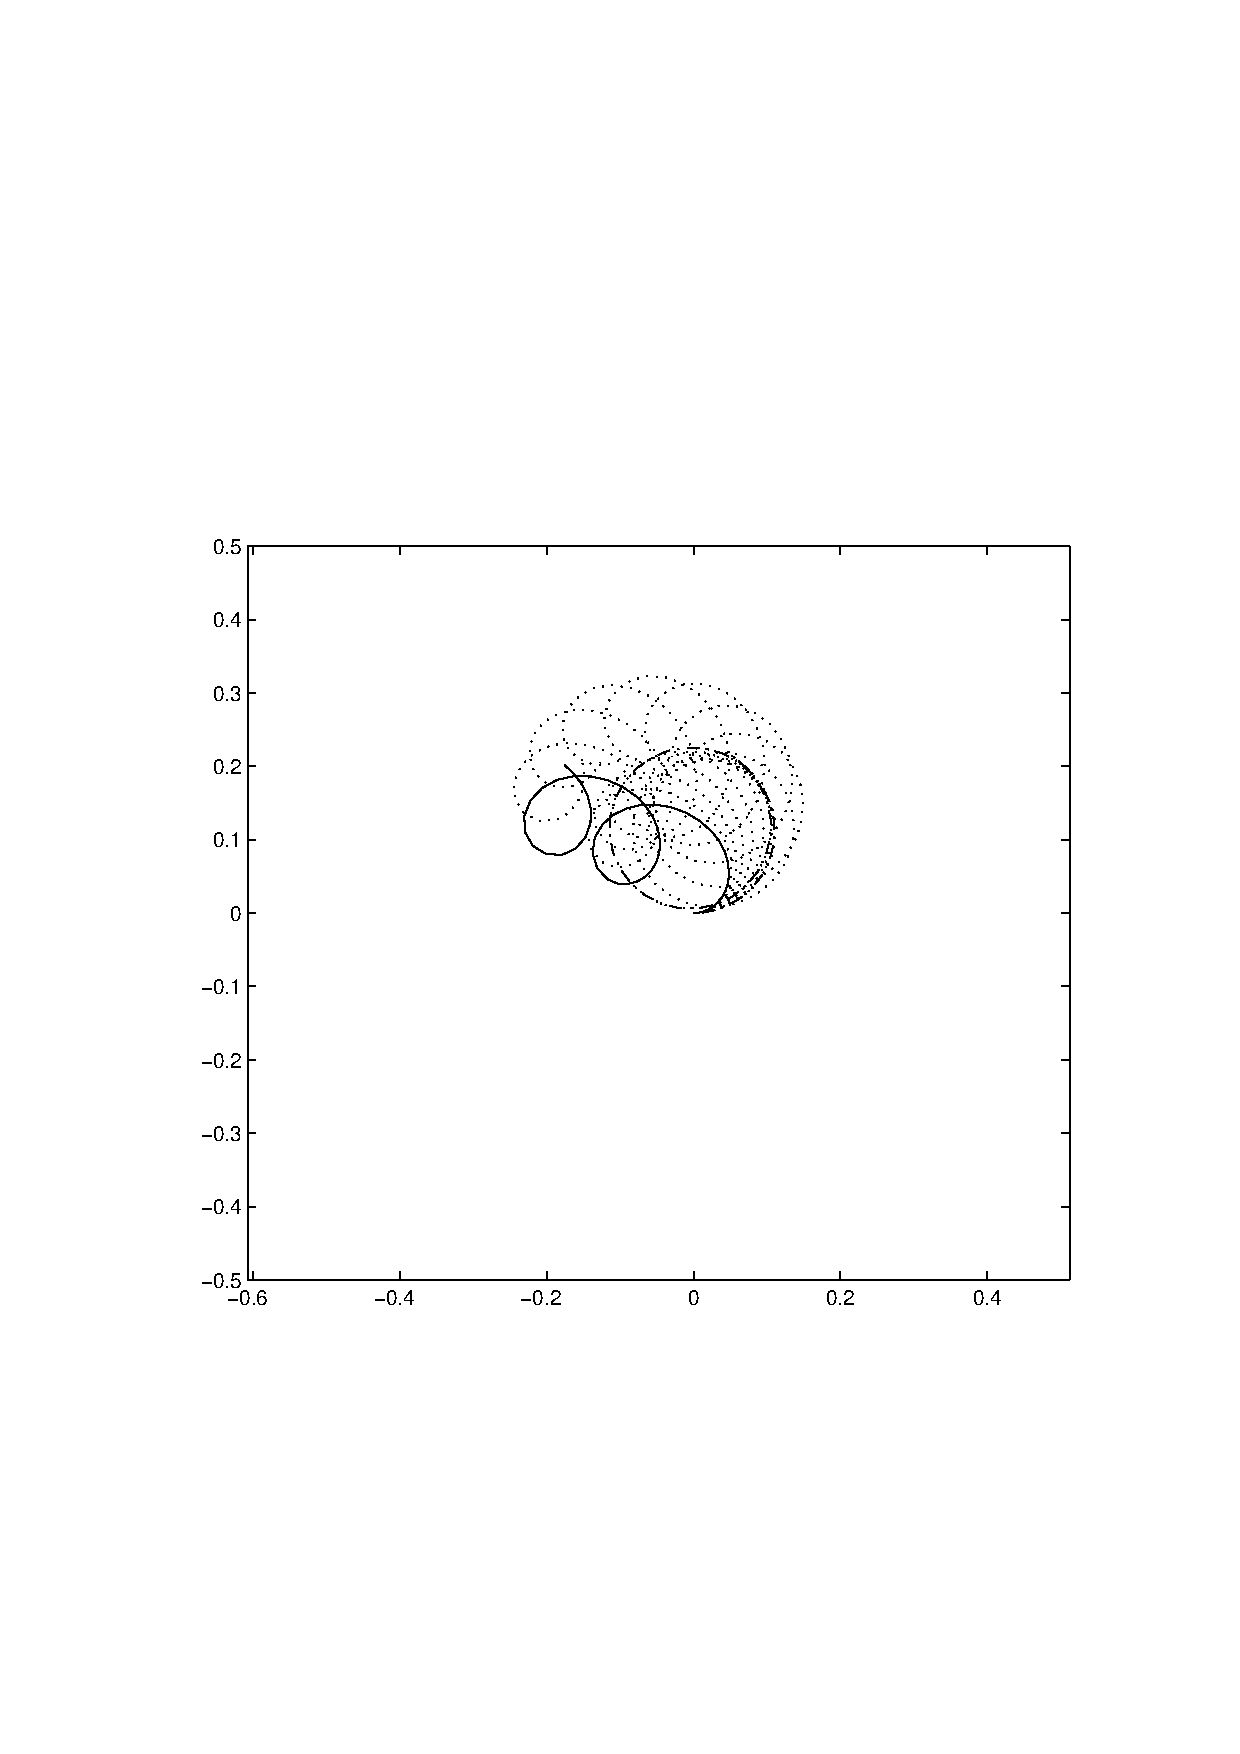
\includegraphics[height=6cm,width=6cm]{dataset2}
\caption{elastic data set 2}
\label{dataset2}
\end{center}
\end{figure} 




%\section{Introduction}
% The very first letter is a 2 line initial drop letter followed
% by the rest of the first word in caps.
% 
% form to use if the first word consists of a single letter:
% \IEEEPARstart{A}{demo} file is ....
% 
% form to use if you need the single drop letter followed by
% normal text (unknown if ever used by the IEEE):
% \IEEEPARstart{A}{}demo file is ....
% 
% Some journals put the first two words in caps:
% \IEEEPARstart{T}{his demo} file is ....
% 
% Here we have the typical use of a "T" for an initial drop letter
% and "HIS" in caps to complete the first word.

% You must have at least 2 lines in the paragraph with the drop letter
% (should never be an issue)


\section{Getexample Outline}

The main aim of the \emph{getexample} is to provide easy access to the examples for the users. For this reason, the getexample tool is expected to be 
have the following design specifications:

\begin{figure}[!ht]
\begin{center}
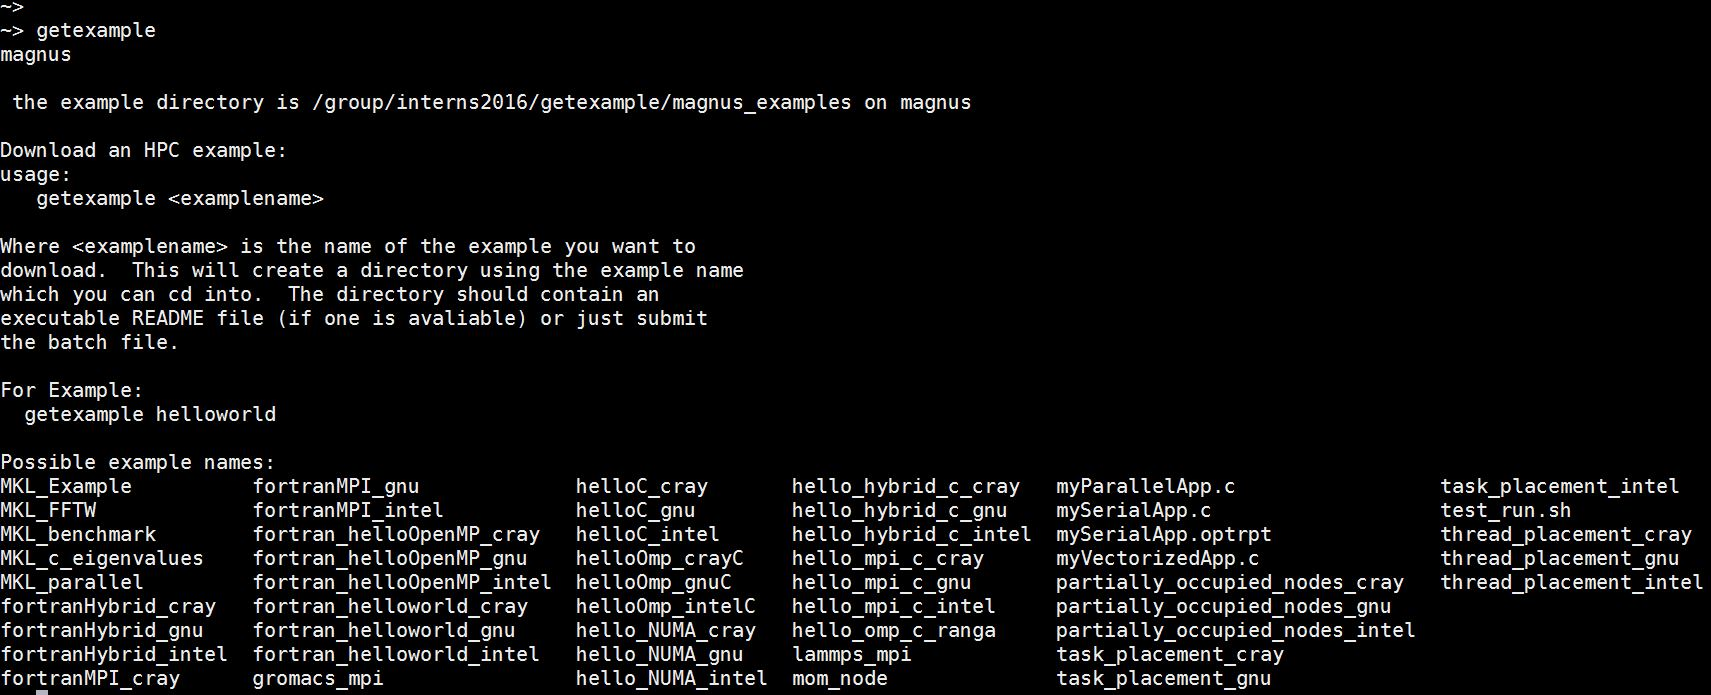
\includegraphics[scale=0.6]{getexample}
\caption{The Listing of Examples when typed "getexample" on Magnus}
%\label{dataset1}
\end{center}
\end{figure}

\begin{figure}[!ht]
\begin{center}
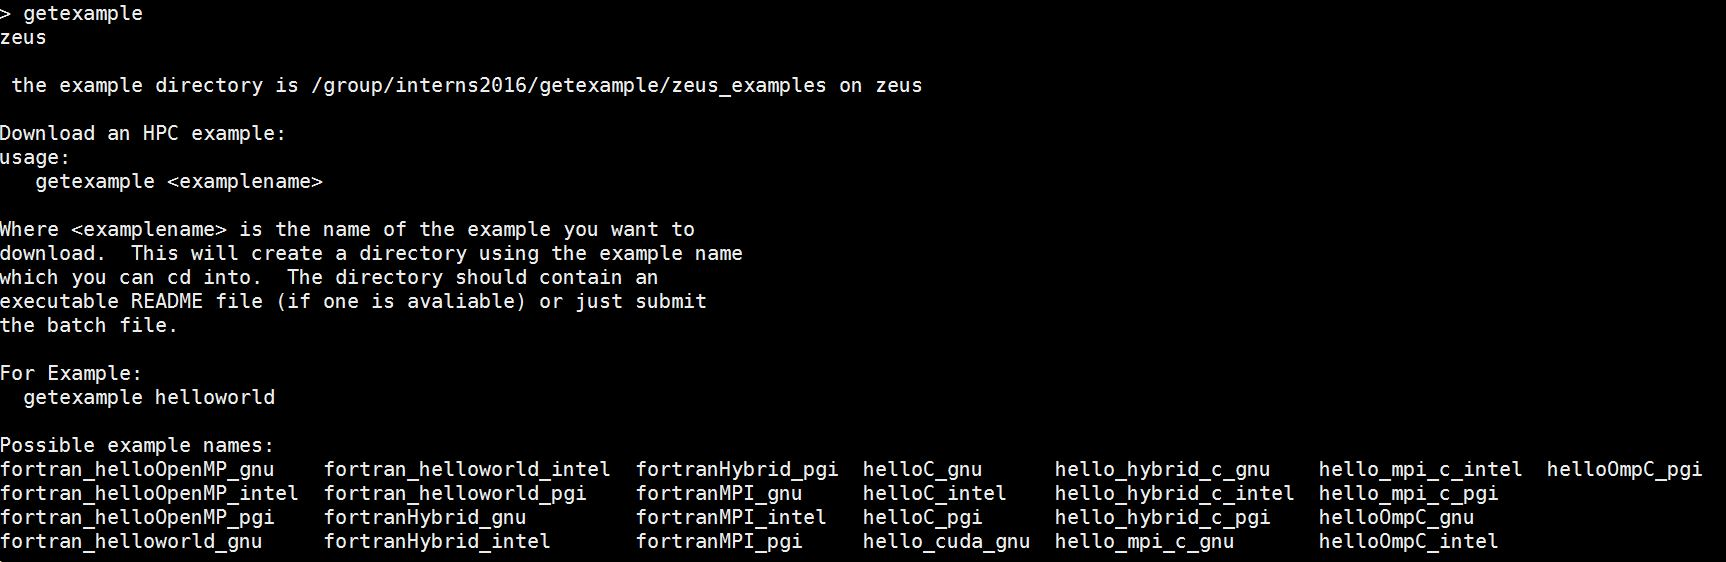
\includegraphics[scale=0.61]{getexamplezeus}
\caption{The Listing of Examples when typed "getexample" on Zeus}
%\label{dataset1}
\end{center}
\end{figure}

\begin{figure}[!ht]
\begin{center}
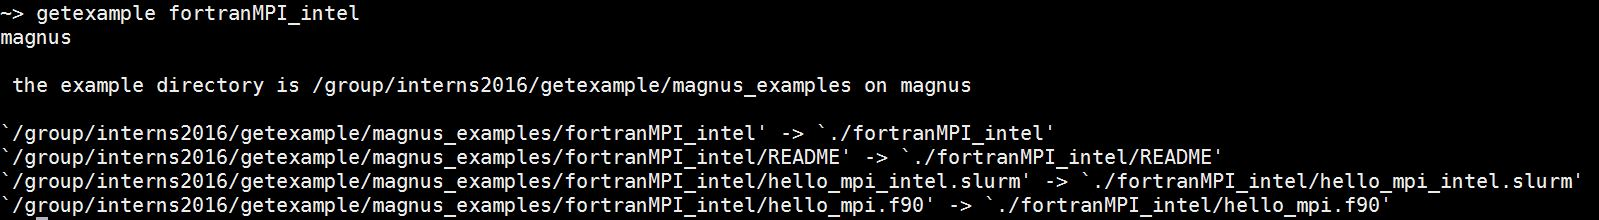
\includegraphics[scale=0.63]{getexamplehybrid}
\caption{Feedback given to the user while downloading the example}
%\label{dataset1}
\end{center}
\end{figure}

\begin{figure}[!ht]
\begin{center}
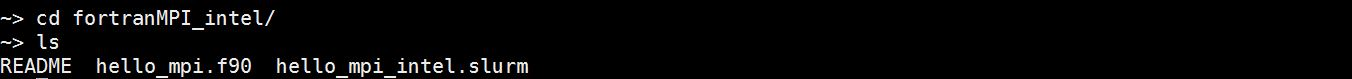
\includegraphics[scale=0.70]{files}
\caption{The List of files in the fortranHybrid\_intel directory}
%\label{dataset1}
\end{center}
\end{figure}

\clearpage

\begin{itemize}
\item It should be easy to use for everyone including beginners. The user should be able to download the examples and run them with one command.
\item It should provide practical examples which can be modified or updated by the users for their own work. Therefore, it encourages the users to learn
how to use the resources given to them effectively.
\item The examples should be clear and completely detailed with steps to help the users understand and apply it.
\end{itemize}

The getexample tool is designed in a way such that when \emph{getexample} command is typed from any directory on the resources of Pawsey Centre, it 
lists all the examples within the getexample library as shown in Fig. 1 on the previous page. As the getexample displays many examples which aim to 
perform various tasks for each individual resource at Pawsey, it ensures that when the user logins from a specific supercomputer such as Magnus, it 
only lists the examples provided for Magnus rather than showing all of the examples within the library. To obtain a copy of any example, the user simply 
types \emph{getexample} followed by the name of the example as shown below:

\begin{tcolorbox}
\begin{Verbatim}[fontsize=\scriptsize]
getexample <name of the example>
\end{Verbatim}
\end{tcolorbox}

This creates a new directory with same name as the example requested in wherever the getexample tool is accessed from and it downloads all the files of
the example to the new directory created and gives a feedback to the user about what the command is doing as shown in Fig. 2. The new directory then can 
be accessed by the user simply typing:

\begin{tcolorbox}
\begin{Verbatim}[fontsize=\scriptsize]
cd <name of the example>
\end{Verbatim}
\end{tcolorbox}

As mentioned earlier, each example consists of 3 files which are the README and SLURM scripts, and the source code as shown in Fig. 3 on the previous
page.




\section{Creating Examples for the Getexample Library}

The examples included in the getexample library were created by the internship students at Pawsey with their supervisor while the source codes within the
getexample were obtained from some wiki pages and websites which were acknowledged in the examples. Some of the examples were also created due to the
needs of research students for their internship projects at Pawsey. The examples obtained in the getexample are mainly for teaching the users how to work
with parallel programming including MPI, OpenMP and hybrid jobs such as OpenMP/MPI which utilise basic source codes similar to \emph{"Hello world"} 
program and submit these jobs to different supercomputers such as Magnus, Zeus and Zythos using different program environments and compiler modules. 

Each individual example on the getexample occupies a directory that is reserved for them and each example consists of three files listed below:

\begin{itemize}    
\item SLURM (Simple Linux Utility for Resource Management) : This allows the users to submit batch jobs to the supercomputers, check on their status and 
cancel them if needed. It contains the necessary information about the name of the executable, the results directory, the name of the output file and 
the jobID. It also allows the users to edit how many nodes the code requires to run on the HPC systems, the duration of the task that it takes, which 
partition to be used and their account name. The SLURM initially creates a scracth directory for the example to run in and the results are outputted to 
a log file. Then, it creates a group directory in which the results directory is located for that example. Once the output file is completed within the 
scratch, the output file is then moved to the results directory located in the group directory and the scratch directory then gets removed.
\item Source Code : This is usually a source code in C or FORTRAN and taken from some wiki pages to run the example.
\item README : This file is an executable Bash script which can be read and run by the users. It provides details about what the source code does,
how to compile the source code depending on the program environment such as Cray, Intel, GNU or compilers like PGI, what can be modified in the SLURM 
directives, and a set of instruction on how to submit the SLURM to the supercomputers including which specific commands to use for particular 
supercomputers. It can be executed by simply typing ./README which then compiles the source code and submits the batch job to the chosen supercomputer.
\end{itemize}

For the examples in the getexample tool to be user friendly, helpful and efficient for working with Pawsey Centre resources, there are many design 
considerations to be held as listed below:

\begin{itemize}
\item Before introducing the examples to the users, it should be ensured that the examples run without encountering any errors. For example,
they should be suitable for the current operating systems with the use of correct commands for the different compiler modules such as Intel, GNU,
and PGI or different program environments such as Cray.
\item All the files to run the example should be included with the example.
\item To minimise confusion on how to perform the example on the supercomputers, the example should be executed with a single command. For example, 
if a simple Bash script is used, it should be run as ./README.
\item The examples should have enough instructions on what each command does and which parts of the SLURM and the README file can be modified so that
all the files and the scripts should be able to edited easily by the users for their preferences. These instructions should be understandable by the new 
users who are not very experienced with these systems. For example, if the user wishes to use more nodes on the supercomputers, one should be able to 
know where to change it from.
\end{itemize}
 
Even though, the examples in the getexample tool are designed in a such way that once they are downloaded, the user should be able to run them without
having to modify them. However, this is not always the case as some of the supercomputers in Pawsey Supercomputing Centre such as Zythos due to
different set ups require the account name which is customized for each user and without the correct account name in the SLURM, the code fails to run. 
Therefore, the examples in the getexample tool ensures that the users are informed on how to change their account name located in the SLURM file.
Furthermore, they assist the users on how to change number of nodes used within the supercomputers and increase or reduce the number of cores used
based on the user's preferences.



\subsection{Magnus}

Magnus is described as a Cray X40 supercomputer that consists of many nodes that are bound by a high speed network. For the compute nodes, each one 
of them has 2 sockets and each of these has 12 cores. Magnus is also specified to have 24 cores per node and in total these sum up to 35,712 cores across 
the 1488 nodes. 

On Magnus, jobs run on the back-end of the system with the help of SLURM and ALPS (the Cray Application Level Placement Scheduler). A batch job is 
submitted to the queue system on the front-end from the sbatch command. When it runs, it executes the launch command aprun on the MOM nodes 
which are the login nodes of Magnus. The aprun keeps running on these login nodes until the application gets completed. Once aprun finishes, the SLURM 
job also completes.

As mentioned previously, the focus of the getexample tool was not only to provide working examples to the users but also assist them on how to run jobs
on their scratch directories. Therefore, whenever the batch job was submitted to Magnus, it was ran on the scracth directory and once the job was 
completed, the results were carried to the group directory. In the end, the scracth was removed. The examples used for Magnus were mainly parallel
programming examples such as MPI, OpenMP and hybrid codes which a combination of OpenMP and MPI tasks and some applications such as LAMMPS and GROMACS.
The source codes used for these examples were written in c or Fortran and were basic \emph{"Hello world"} codes with the exception of the application codes.
Each example was displayed in different environments on Magnus such as GNU, Intel and more importantly the default environment, Cray with the compiler
options of ftn, mpif90 and cc. When using these environments, it was important to load the actual programming environment before compiling the source
codes and running them as each environment has specific compiler commands with distinct wrappers.


\subsubsection{MPI Examples}

MPI is known as a Message Passing Interface application that is a communication model for moving data between processors. For MPI examples, FORTRAN and 
C codes were mainly used and ran on different environments including Cray, GNU and Intel. On Magnus, the default program environment is Cray. Therefore, 
it was necessary to load each program environment that was intended to work on by doing a:

\begin{tcolorbox}
\begin{Verbatim}[fontsize=\scriptsize]
module swap PrgEnv-cray PrgEnv-<name of the environment>
\end{Verbatim}
\end{tcolorbox}

It is also very important to notice that if the right program environment is not loaded, the code will fail as each environment have different commands 
for compilers. However, on Magnus, swapping from one environment to the other might be very challenging for the new users. As the getexample tool is
desired to be as automated as possible to minimise failures on tasks, it was made sure that after running each job on Intel and GNU environments, the
environment was set back to the default environment, Cray. This prevents the users to manually list the module every time they run something on Magnus
and modify the codes to swap from one module to the other. 

The very first MPI example performed on Magnus ran on 2 nodes with a total of 48 tasks with a basic \emph{"Hello world"} source code in both C and FORTRAN. 
This example consisted of three files as mentioned previously which were README, SLURM and the source code. The SLURM script included information about
the choice in the number of nodes, the partition, the duration of the time it takes to run the job, where to run the task such as on scratch and where
to store the results, for example the group. It also specified the name of the executable, the results directory and the output file. 

For the getexample on Magnus, the classified partition is the debugq. Since, there were 2 nodes used, the SLURM directives were given as:

\begin{tcolorbox}
\begin{Verbatim}[fontsize=\scriptsize]
#!/bin/bash -l
#SBATCH --job-name=GE-hostname
#SBATCH --partition=debugq
#SBATCH --nodes=2
#SBATCH --time=00:05:00
#SBATCH --export=NONE
\end{Verbatim}
\end{tcolorbox}

The generic variables such as the executable, scratch, the results directory and the output file were defined as shown below:

\begin{tcolorbox}
\begin{Verbatim}[fontsize=\scriptsize]
EXECUTABLE=hello_mpi_cray
SCRATCH=$MYSCRATCH/run_hostname/$SLURM_JOBID
RESULTS=$MYGROUP/mpifortran_cray_results/$SLURM_JOBID

OUTPUT=mpifortran_cray.log 
\end{Verbatim}
\end{tcolorbox}

To launch the MPI job with fully occupied 2 nodes, the aprun command was used as expressed:

\begin{tcolorbox}
\begin{Verbatim}[fontsize=\scriptsize]
aprun -n 48 -N 24 ./$EXECUTABLE >> ${OUTPUT}
\end{Verbatim}
\end{tcolorbox}

where -n defines the total number of MPI tasks while -N specifies the number of MPI tasks per node as there are 2 nodes.

In the README file, the correct program environment should be included for the codes to run well. For compiling on Cray, there was no need to load
this environment as the default module was Cray. However, to run on GNU and Intel, the program environment was changed from Cray to GNU or Intel as
shown below:

\begin{tcolorbox}
\begin{Verbatim}[fontsize=\scriptsize]
module swap PrgEnv-cray PrgEnv-gnu
module swap PrgEnv-cray PrgEnv-intel
\end{Verbatim}
\end{tcolorbox}

However, the compiler commands do not change for Cray, GNU and Intel for MPI codes on Magnus, whereas they have distinct differences for other parallel
programming tasks such as OpenMP.

To compile the \emph{"Hello world"} MPI FORTRAN code, hello\_mpi.f90 on Cray, GNU and Intel environments:

\begin{tcolorbox}
\begin{Verbatim}[fontsize=\scriptsize]
ftn -O2 hello_mpi.f90 -o hello_mpi_cray
\end{Verbatim}
\end{tcolorbox}

-O2 is the optimization method, while -o placed after the source code directs to an executable called hello\_mpi\_cray which was previously defined in
the SLURM and chosen by the technical staff as a name. For GNU and Intel, this was called hello\_mpi\_gnu and hello\_mpi\_intel. 

When the source code was in C, the SLURM was not different from that of FORTRAN. However, the README did change. To compile the hello\_mpi.c code, the 
following command was used: 

\begin{tcolorbox}
\begin{Verbatim}[fontsize=\scriptsize]
cc -O2 hello_mpi.c -o hello_mpi_cray
\end{Verbatim}
\end{tcolorbox}

Once the codes were compiled, the SLURM was then submitted to Magnus by:

\begin{tcolorbox}
\begin{Verbatim}[fontsize=\scriptsize]
sbatch hello_mpi_cray.slurm 
\end{Verbatim}
\end{tcolorbox}

As mentioned earlier, to prevent the users from manually listing the modules to see which modules are loaded and from which module to swap, at the end
of the SLURM and the README, the program environment was always set back to the default by:

\begin{tcolorbox}
\begin{Verbatim}[fontsize=\scriptsize]
module swap PrgEnv-<name of the environment> PrgEnv-cray
\end{Verbatim}
\end{tcolorbox}

Another example on MPI was to run the same sources but on partially occupied nodes which means that instead of having 24 tasks per node, each node could
only have 12 tasks. When running this example on Magnus, the README remained unchanged, but there were minor changes to the SLURM.

The number of OpenMP threads was set to 1 to prevent from inadvertent OpenMP threading and the aprun command was changed to:

\begin{tcolorbox}
\begin{Verbatim}[fontsize=\scriptsize]
aprun -n 24 -N 12 -S 6 ./$EXECUTABLE >> ${OUTPUT}
\end{Verbatim}
\end{tcolorbox}

-n defines the total number of MPI tasks, -N specifies the number tasks per node while -S defines the number of MPI tasks per socket.



\subsubsection(Hybrid Examples}

A hybrid job is a mixed job that is a combination of OpenMP and MPI tasks. It aims to take advantage of the OpenMP in NUMA region which is also known as 
a socket. The NUMA region was in this case involved with one 12-core chip and ran on 6 threads on each of 8 MPI tasks which dispersed evenly between 
the NUMA regions.A sum of 2 nodes was required which accomodated 8 MPI tasks and 6 threads. Besides specifying the number of nodes, the time was also shown in the slurm 
script as done in the previous examples. In this case, we chose 5 minutes as done in most of the examples in the getexample.
The partition remains the same debugq.


\begin{tcolorbox}
\begin{verbatim}
#SBATCH --partition=debugq
#SBATCH --nodes=2
#SBATCH --time=00:05:00
#SBATCH --export=NONE
\end{verbatim}
\end{tcolorbox}

8 MPI tasks (-n 8) were specified to aprun to launch the job with 4 MPI tasks per node (-N 4), 2 MPI tasks per socket (-S 6) and each of the 8 MPI tasks 
had 6 OpenMP threads (-d 6). Therefore, the number of OpenMP threads, {OMP\_NUM\_THREADS} was set to 6.
This full expression is shown as:

\begin{tcolorbox}
\begin{Verbatim}[fontsize=\stripsize]
export OMP_NUM_THREADS=6
aprun -n 8 -N 4 -S 2 -d 6 ./$EXECUTABLE >> ${OUTPUT}
\end{Verbatim}
\end{tcolorbox}

Once again, to run on multiple threads with the Intel environment on Cray, AFFINITY should be disabled with the same command used in the OpenMP examples
just after the aprun command.The source codes used for the hybrid examples were also consisted of both Fortran and c which were hybrid\_hello.f90 and hello\_hybrid.c. The README 
script contained the compiling commands to compile on Cray as shown below :

\begin{tcolorbox}
\begin{Verbatim}[fontsize=\stripsize]
ftn -O2 -h omp hybrid_hello.f90 -o hello_hybrid_cray for the Fortran code
cc -O2 -h omp hybrid_hello.c -o hello_hybrid_cray for the c code
\end{Verbatim}
\end{tcolorbox}

To compile with the GNU environment for fortran and c codes respectively, the README had the following compilers:

\begin{tcolorbox}
\begin{Verbatim}[fontsize=\stripsize]
ftn -O2 -fopenmp hybrid_hello.f90 -o hello_hybrid_gnu
cc -O2 -fopenmp hybrid_hello.c -o hello_hybrid_gnu
\end{Verbatim}
\end{tcolorbox}

For the intel environment, the compiler code changes to:

\begin{tcolorbox}
\begin{Verbatim}[fontsize=\stripsize]
ftn -O2 -openmp hybrid_hello.f90 -o hello_hybrid_intel
cc -O2 -openmp hybrid_hello.c -o hello_hybrid_intel
\end{Verbatim}
\end{tcolorbox}

The same sbatch command as the OpenMP and MPI tasks was used for the hybrid codes to submit them to Magnus. The only difference was the name of the name
of the SLURM scripts.



\subsection{lammps}

\begin{Verbatim}[fontsize=\stripsize]
LAMMPS <is a traditional molecular dynamics code
\end{Verbatim} 

It is also an acronym for Large-scale Atomic/Molecular Massively Parallel Simulator. It has potentials
for solid state materials which include metals and semicoductors. It also has potential for delicate matter i.e biomolecules and polymers and also
coarse-grained or mesoscopic systems.

LAMMPS is an easy tool used to model atoms or rather, as a parallel molecule test simulator at the atomic, meso, or continuum scale. This tool runs on
single processors or in parallel making the use of message-passing systems (MPI) and a spatial-decomposition of the simulator domain. A significant
number of its models have forms that give accelerated performance on CPUs, GPUs, and Intel Xeon Phi processors.

The LAMMPS example done in the getexample tool was specifically run on Magnus. The source code had been provided with a large number of atoms and their
properties and potentials. The existing SLURM file of the MPI tasks of Magnus was utilized and modified to request a total of 2 nodes. The partition
remained as debugq as it is the correct partition for Magnus. The time was changed to 20 minutes as an increase in time would be better because it gives
sufficient time to run the code. If the time is not long enough, it does not completely run the code and kills the job once the time runs out.
The two files epm2.lmp  epm2data.lmp  lammps_mpi_gnu.slurm

The following commads show the SLURM directives needed for the LAMMPS task:

\begin{tcolorbox}
\begin{verbatim}
\hyphenation{#-!-/-bin-/bash -l}
#SBATCH --job-name=hostname
#SBATCH --partition=debugq
#SBATCH --nodes=2
#SBATCH --time=00:20:00
#SBATCH --export=NONE
\end{verbatim}
\end{tcolorbox}

The program environment used for this task was GNU, hence the module was swapped from Cray to GNU and and the lammps module was loaded which is required
to run the source code and the data.

\begin{tcolorbox}
\begin{verbatim}
swap PrgEnv-cray PrgEnv-gnu
load lammps
\end{verbatim}
\end{tcolorbox}

In the template of the SLURM, an executable, a results directory and an output were declared to store the results of the LAMMPS example in the group filenames below:

\begin{tcolorbox}
\begin{Verbatim}[fontsize=\scriptsize]
EXECUTABLE=lmp_mpi
SCRATCH=$MYSCRATCH/run_lammps/$SLURM_JOBID
RESULTS=$MYGROUP/lmp_mpi_results/$SLURM_JOBID
\end{Verbatim}
\end{tcolorbox}

Before running the example on the SCRATCH, the files ending with .lmp name which contain the data and code were copied to the SCRACTH and this was
obtained in the SLURM as:

\begin{tcolorbox}
\begin{verbatim}
cp *.lmp $SCRATCH
\end{verbatim}
\end{tcolorbox}

As this LAMMPS example is an MPI task, it was run on Magnus on 2 nodes with 24 MPI tasks per node giving a total of 48 tasks and this was implemented
with the aprun command to launch:

\begin{tcolorbox}
\begin{Verbatim}[fontsize=\scriptsize]
\aprun -n 48 -N 24 $EXECUTABLE < epm2.lmp >> ${OUTPUT}
\end{Verbatim}
\end{tcolorbox}


The SLURM was submitted to Magnus by the identical sbatch command used in the README files of all the Magnus examples.



%\hfill mds
 
%\hfill August 26, 2015

%\subsection{Subsection Heading Here}
%Subsection text here.

% needed in second column of first page if using \IEEEpubid
%\IEEEpubidadjcol

%\subsubsection{Subsubsection Heading Here}
%Subsubsection text here.


% An example of a floating figure using the graphicx package.
% Note that \label must occur AFTER (or within) \caption.
% For figures, \caption should occur after the \includegraphics.
% Note that IEEEtran v1.7 and later has special internal code that
% is designed to preserve the operation of \label within \caption
% even when the captionsoff option is in effect. However, because
% of issues like this, it may be the safest practice to put all your
% \label just after \caption rather than within \caption{}.
%
% Reminder: the "draftcls" or "draftclsnofoot", not "draft", class
% option should be used if it is desired that the figures are to be
% displayed while in draft mode.
%
%\begin{figure}[!t]
%\centering
%\includegraphics[width=2.5in]{myfigure}
% where an .eps filename suffix will be assumed under latex, 
% and a .pdf suffix will be assumed for pdflatex; or what has been declared
% via \DeclareGraphicsExtensions.
%\caption{Simulation results for the network.}
%\label{fig_sim}
%\end{figure}

% Note that the IEEE typically puts floats only at the top, even when this
% results in a large percentage of a column being occupied by floats.


% An example of a double column floating figure using two subfigures.
% (The subfig.sty package must be loaded for this to work.)
% The subfigure \label commands are set within each subfloat command,
% and the \label for the overall figure must come after \caption.
% \hfil is used as a separator to get equal spacing.
% Watch out that the combined width of all the subfigures on a 
% line do not exceed the text width or a line break will occur.
%
%\begin{figure*}[!t]
%\centering
%\subfloat[Case I]{\includegraphics[width=2.5in]{box}%
%\label{fig_first_case}}
%\hfil
%\subfloat[Case II]{\includegraphics[width=2.5in]{box}%
%\label{fig_second_case}}
%\caption{Simulation results for the network.}
%\label{fig_sim}
%\end{figure*}
%
% Note that often IEEE papers with subfigures do not employ subfigure
% captions (using the optional argument to \subfloat[]), but instead will
% reference/describe all of them (a), (b), etc., within the main caption.
% Be aware that for subfig.sty to generate the (a), (b), etc., subfigure
% labels, the optional argument to \subfloat must be present. If a
% subcaption is not desired, just leave its contents blank,
% e.g., \subfloat[].


% An example of a floating table. Note that, for IEEE style tables, the
% \caption command should come BEFORE the table and, given that table
% captions serve much like titles, are usually capitalized except for words
% such as a, an, and, as, at, but, by, for, in, nor, of, on, or, the, to
% and up, which are usually not capitalized unless they are the first or
% last word of the caption. Table text will default to \footnotesize as
% the IEEE normally uses this smaller font for tables.
% The \label must come after \caption as always.
%
%\begin{table}[!t]
%% increase table row spacing, adjust to taste
%\renewcommand{\arraystretch}{1.3}
% if using array.sty, it might be a good idea to tweak the value of
% \extrarowheight as needed to properly center the text within the cells
%\caption{An Example of a Table}
%\label{table_example}
%\centering
%% Some packages, such as MDW tools, offer better commands for making tables
%% than the plain LaTeX2e tabular which is used here.
%\begin{tabular}{|c||c|}
%\hline
%One & Two\\
%\hline
%Three & Four\\
%\hline
%\end{tabular}
%\end{table}


% Note that the IEEE does not put floats in the very first column
% - or typically anywhere on the first page for that matter. Also,
% in-text middle ("here") positioning is typically not used, but it
% is allowed and encouraged for Computer Society conferences (but
% not Computer Society journals). Most IEEE journals/conferences use
% top floats exclusively. 
% Note that, LaTeX2e, unlike IEEE journals/conferences, places
% footnotes above bottom floats. This can be corrected via the
% \fnbelowfloat command of the stfloats package.




\section{Conclusion}
The conclusion goes here.





% if have a single appendix:
%\appendix[Proof of the Zonklar Equations]
% or
%\appendix  % for no appendix heading
% do not use \section anymore after \appendix, only \section*
% is possibly needed

% use appendices with more than one appendix
% then use \section to start each appendix
% you must declare a \section before using any
% \subsection or using \label (\appendices by itself
% starts a section numbered zero.)
%


\appendices
\section{Proof of the First Zonklar Equation}
Appendix one text goes here.

% you can choose not to have a title for an appendix
% if you want by leaving the argument blank
\section{}
Appendix two text goes here.


% use section* for acknowledgment
\section*{Acknowledgment}


The authors would like to thank...


% Can use something like this to put references on a page
% by themselves when using endfloat and the captionsoff option.
\ifCLASSOPTIONcaptionsoff
  \newpage
\fi



% trigger a \newpage just before the given reference
% number - used to balance the columns on the last page
% adjust value as needed - may need to be readjusted if
% the document is modified later
%\IEEEtriggeratref{8}
% The "triggered" command can be changed if desired:
%\IEEEtriggercmd{\enlargethispage{-5in}}

% references section

% can use a bibliography generated by BibTeX as a .bbl file
% BibTeX documentation can be easily obtained at:
% http://mirror.ctan.org/biblio/bibtex/contrib/doc/
% The IEEEtran BibTeX style support page is at:
% http://www.michaelshell.org/tex/ieeetran/bibtex/
%\bibliographystyle{IEEEtran}
% argument is your BibTeX string definitions and bibliography database(s)
%\bibliography{IEEEabrv,../bib/paper}
%
% <OR> manually copy in the resultant .bbl file
% set second argument of \begin to the number of references
% (used to reserve space for the reference number labels box)
\begin{thebibliography}{1}

\bibitem{IEEEhowto:kopka}
H.~Kopka and P.~W. Daly, \emph{A Guide to \LaTeX}, 3rd~ed.\hskip 1em plus
  0.5em minus 0.4em\relax Harlow, England: Addison-Wesley, 1999.

\end{thebibliography}

% biography section
% 
% If you have an EPS/PDF photo (graphicx package needed) extra braces are
% needed around the contents of the optional argument to biography to prevent
% the LaTeX parser from getting confused when it sees the complicated
% \includegraphics command within an optional argument. (You could create
% your own custom macro containing the \includegraphics command to make things
% simpler here.)
%\begin{IEEEbiography}[{\includegraphics[width=3cm,height=3.25cm,
%    clip,keepaspectratio]{./pdf/Journal_RCB}}]{Ralph Christopher Bording}
% or if you just want to reserve a space for a photo:

\begin{IEEEbiography}{Ralph Bording}
Biography text here.
\end{IEEEbiography}

% if you will not have a photo at all:
%\begin{IEEEbiographynophoto}{John Doe}
%Biography text here.
%end{IEEEbiographynophoto}

% insert where needed to balance the two columns on the last page with
% biographies
\newpage

\begin{IEEEbiographynophoto}{Jane Doe}
Biography text here.
\end{IEEEbiographynophoto}

% You can push biographies down or up by placing
% a \vfill before or after them. The appropriate
% use of \vfill depends on what kind of text is
% on the last page and whether or not the columns
% are being equalized.

%\vfill

% Can be used to pull up biographies so that the bottom of the last one
% is flush with the other column.
%\enlargethispage{-5in}



% that's all folks
\end{document}


